\documentclass[12pt,a4paper]{report}

% ---------- PACKAGES ----------
\usepackage[utf8]{inputenc}
\usepackage[T1]{fontenc}
\usepackage{lmodern}
\usepackage{setspace}        % line spacing
\usepackage{geometry}        % page margins
\usepackage{booktabs}        % tables
\usepackage{graphicx}        % figures
\usepackage{amsmath, amssymb} % math
\usepackage{hyperref}        % clickable links
\usepackage{natbib}          % bibliography
\usepackage{float}           % tables/figures positioning
\usepackage{caption}
\usepackage{subcaption}
\usepackage{rotating}
\usepackage{listings}
\usepackage{xcolor}

\lstdefinestyle{cmd}{
    basicstyle=\ttfamily\scriptsize, % very small monospace
    lineskip=-1pt,
    aboveskip=10pt,
    belowskip=10pt,
    frame=single,
    breaklines=true,
    showstringspaces=false,
    xleftmargin=1em,
    xrightmargin=1em,
    framexleftmargin=1em,
    framexrightmargin=1em,
}
% --- JSON style ---
\lstdefinestyle{json}{
    basicstyle=\ttfamily\footnotesize,
    keywordstyle=\color{uniRed},
    stringstyle=\color{uniBlue},
    commentstyle=\color{uniGray}\itshape,
    showstringspaces=false,
    breaklines=true,
    frame=single,
    literate=
     *{0}{{{\color{uniRed}0}}}{1}
      {1}{{{\color{uniRed}1}}}{1}
      {2}{{{\color{uniRed}2}}}{1}
      {3}{{{\color{uniRed}3}}}{1}
      {4}{{{\color{uniRed}4}}}{1}
      {5}{{{\color{uniRed}5}}}{1}
      {6}{{{\color{uniRed}6}}}{1}
      {7}{{{\color{uniRed}7}}}{1}
      {8}{{{\color{uniRed}8}}}{1}
      {9}{{{\color{uniRed}9}}}{1}
}

% --- Database Schema / SQL style ---
\lstdefinestyle{db}{
    basicstyle=\ttfamily\footnotesize,
    keywordstyle=\color{uniRed}\bfseries,
    stringstyle=\color{uniBlue},
    commentstyle=\color{uniGray}\itshape,
    numbers=left,
    numberstyle=\tiny\color{uniGray},
    stepnumber=1,
    numbersep=8pt,
    showstringspaces=false,
    breaklines=true,
    frame=single,
    tabsize=2,
    morekeywords={CREATE, TABLE, PRIMARY, KEY, FOREIGN, REFERENCES, VARCHAR, INT, DATE}
}

% --- Python style ---
\lstdefinestyle{python}{
    basicstyle=\ttfamily\footnotesize,
    keywordstyle=\color{uniRed}\bfseries,
    stringstyle=\color{uniBlue},
    commentstyle=\color{uniGray}\itshape,
    numbers=left,
    numberstyle=\tiny\color{uniGray},
    stepnumber=1,
    numbersep=8pt,
    showstringspaces=false,
    breaklines=true,
    frame=single,
    tabsize=4,
    captionpos=b
}


\definecolor{uniRed}{HTML}{E30613}
\definecolor{uniBlue}{HTML}{009FE3}
\definecolor{uniGray}{HTML}{7D7D7D}


\geometry{margin=1.2in}
\doublespacing

% ---------- DOCUMENT ----------
\begin{document}

    \begin{titlepage}
    \centering

    % University Logo
    
\includegraphics[width=0.4\textwidth]{img/unilu_logo}\par\vspace{1cm}
    \vspace{0.5cm}

    % University Name
    {\Large \textbf{Master in Quantitative Economics and Finance} \par}
    \vspace{1cm}

    % Thesis Title
    {\LARGE \bfseries Generating Beliefs for Private Equity using Large Language Models \par}
    \vspace{1cm}

    % Author
    {\Large Leonardo Cruciani \par}
    \vspace{0.5cm}

    % Supervisors
    {\large Relator: Prof.~B. Holcblat \par}
    {\large Co-Relator: Dr.~A. Ermakov \par}
    \vspace{0.5cm}

    % Academic Year
    {\large Academic Year 2024--2025 \par}
    \vspace{1cm}

    % Footer
    \vfill
    {\large Master Thesis \par}
    % Date
    {\large \today \par}
\end{titlepage}

\newpage
\thispagestyle{empty}
\mbox{}
\newpage


\tableofcontents
\newpage

% ===============================

\chapter{Introduction}\label{ch:introduction}
\section{Motivation}\label{sec:motivation}

Private equity (PE) has experienced remarkable growth over the past two decades, emerging as a dominant force in institutional portfolios.
Global assets under management in PE exceeded USD 17 trillion in 2024 (see~\ref{fig:aum_drypowder}), with pension funds, sovereign wealth funds, and endowments allocating an increasing share of capital to the asset class.
This expansion is driven by the promise of superior returns and diversification benefits; however, PE remains fundamentally different from public markets.
Valuations are opaque, transactions are infrequent, and information is primarily controlled by general partners (GPs) through periodic reporting.
These features make it difficult to determine whether observed performance reflects true skill or risk-taking, and they place investor beliefs at the center of capital allocation decisions.

\begin{figure}[H]
    \centering
    \begin{subfigure}{0.48\textwidth}
        \centering
        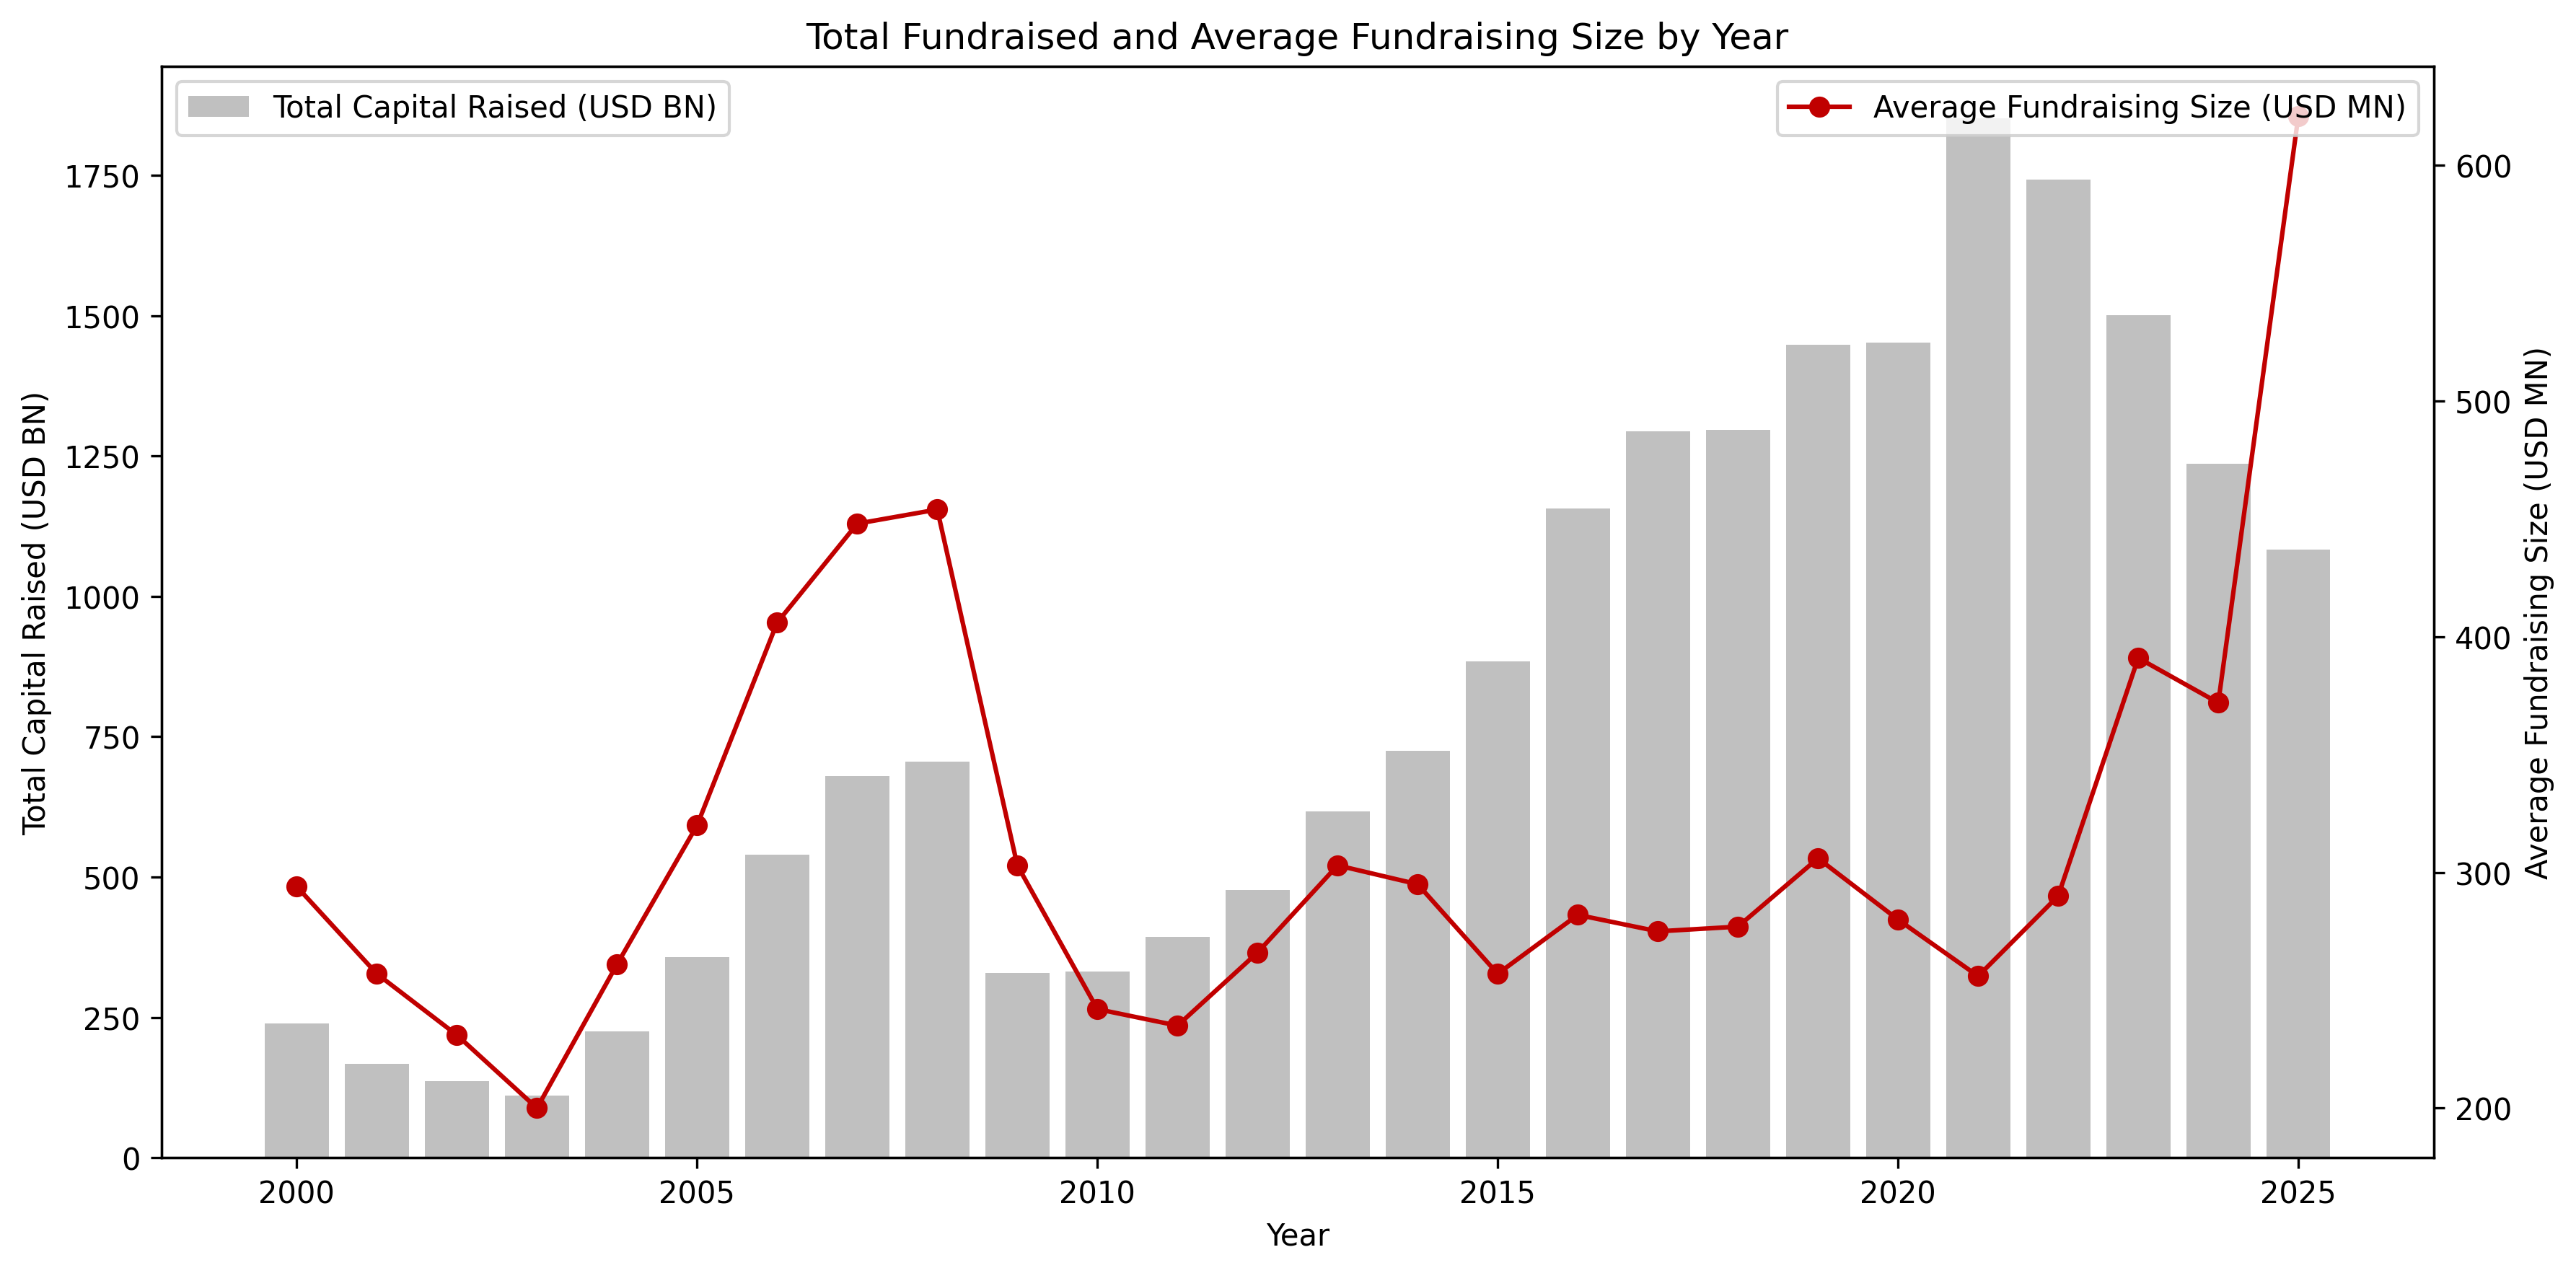
\includegraphics[width=\linewidth]{img/fundraising_vs_average}
        \caption{Private equity fundraising and average deal size.}
        \label{fig:fundraising}
    \end{subfigure}
    \hfill
    \begin{subfigure}{0.48\textwidth}
        \centering
        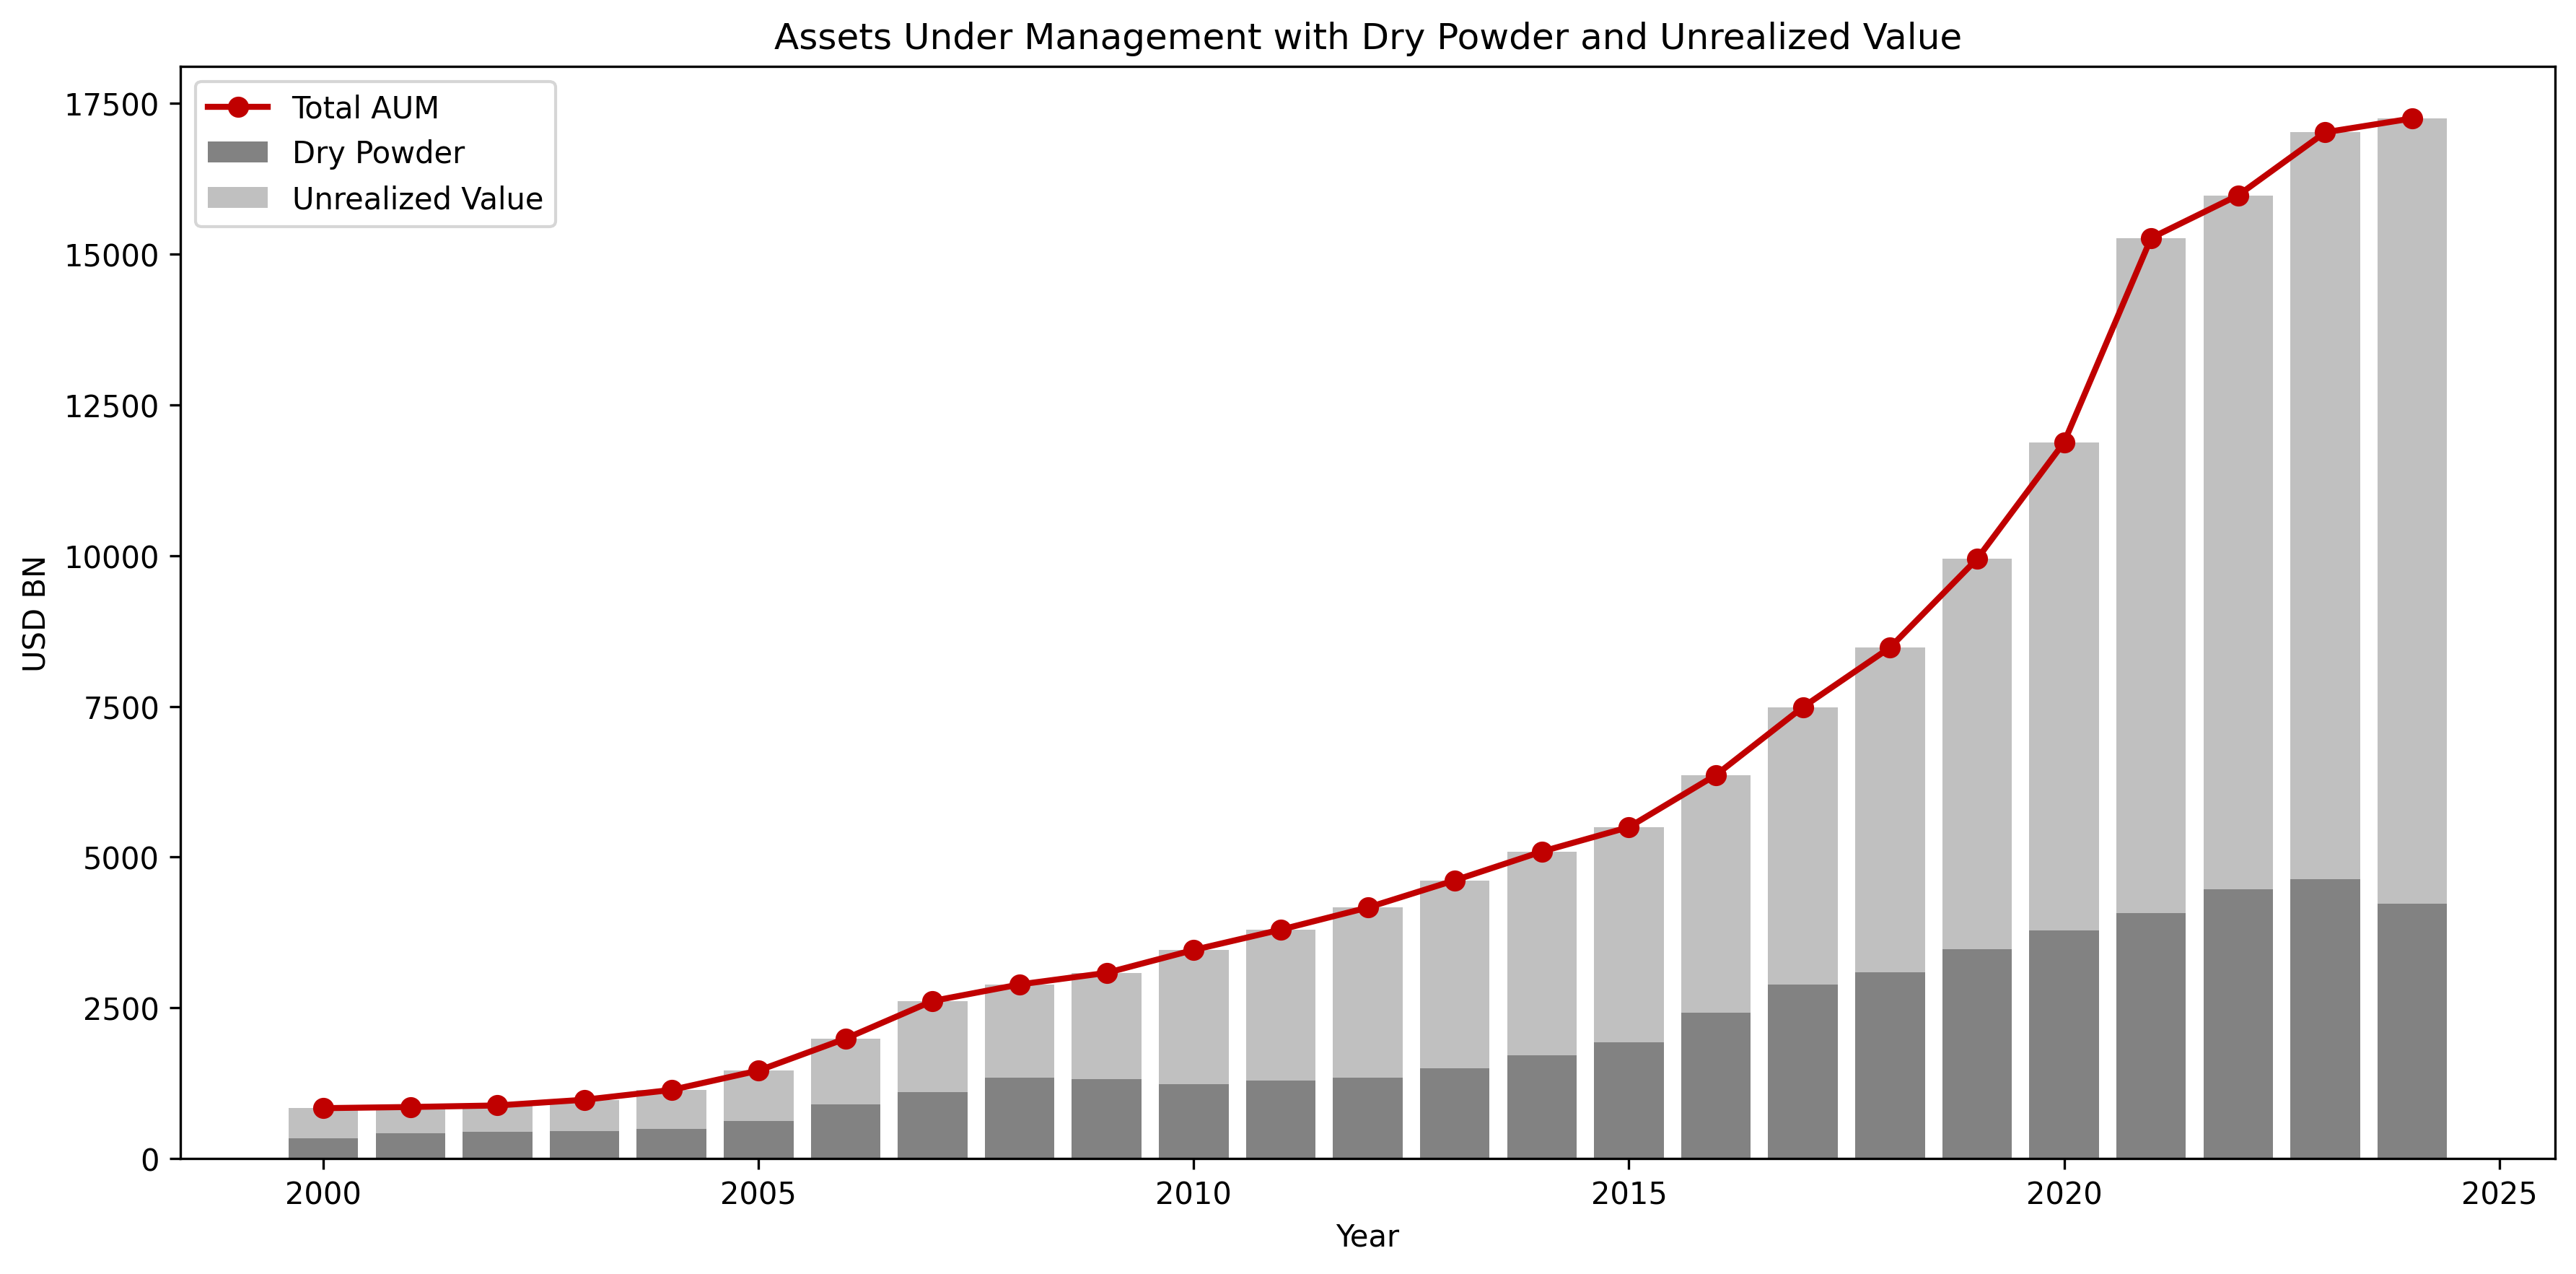
\includegraphics[width=\linewidth]{img/aum_drypowder_unrealized}
        \caption{PE assets under management, dry powder, and unrealized value.}
        \label{fig:aum_drypowder}
    \end{subfigure}
    \caption{Trends in private equity cash flows and capital. Data from Preqin.}
    \label{fig:pe_trends}
\end{figure}

In fact, unlike public equities, where investor beliefs can be inferred directly from market prices, private equity beliefs are not observable in real time.
Limited partners (LPs) form expectations about future distributions, exit values, and returns by interpreting a narrow set of signals: GP reports, due diligence materials, industry news, and historical cash flows.
GP communications often combine hard information with softer language that can influence perceptions, and it remains unclear whether LPs are consistently able to extract the predictive content of these narratives or if they are sometimes influenced by sentiment and bias.
Historical episodes illustrate the stakes: during the global financial crisis (2008-2009), many PE funds were slow to revise net asset values (NAVs), creating a disconnect between reported valuations and underlying fundamentals.
In contrast, during the COVID-19 shock, GPs initially issued cautious updates but quickly turned more optimistic as public markets recovered.
Both episodes suggest that GP communications can shape investor beliefs in ways not fully explained by fundamentals, with potential implications for capital allocation and risk perception (see Figure~\ref{fig:pe_vs_pm}).

\begin{figure}
    \centering
    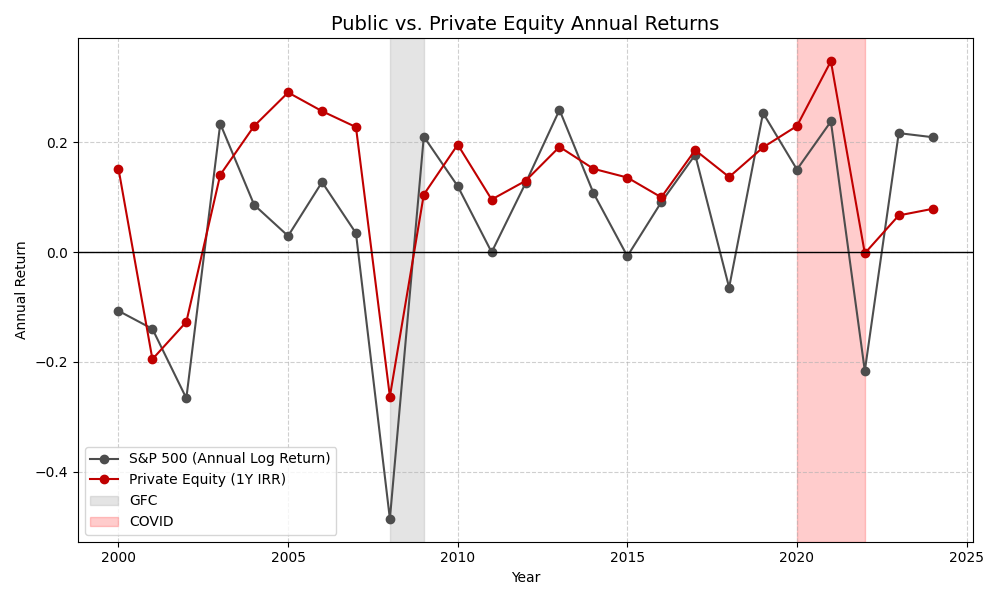
\includegraphics[width=0.8 \linewidth]{img/pe_vs_pm}
    \caption{Private equity returns (source: Preqin) are calculated using the NAV reported by GPs. Therefore, they tend to be much less elastic than market returns.}
    \label{fig:pe_vs_pm}
\end{figure}

Recent advances in natural language processing (NLP) and the emergence of large language models (LLMs) offer a new lens to examine these dynamics.
LLMs can process complex textual information and generate probabilistic forecasts based on contextual cues, mimicking or even surpassing human
interpretation.
In public markets, LLMs have already been shown to match human analysts performances when it comes to predict returns, infer sentiment, and identify risk exposures from unstructured data.
However, private markets present a more challenging environment: the data is scarcer, disclosures are less standardized, and outcomes are realized over long horizons.
The aim of this thesis is to introduce a methodology to use LLMs to process GPs report to extract information effectively and quantify the sentiment expressed by these documents.

\section{Literature Review}\label{sec:literature-review}

Classical models assume rational expectations, where investors form unbiased forecasts given available information.
Yet empirical evidence shows that beliefs often deviate systematically from fundamentals.
Behavioral models document patterns such as overreaction to recent performance, underreaction to fundamentals, and herding behavior~\citep{barberis2018behavioral}, observed in analyst forecasts, mutual fund flows, and investor reactions to earnings announcements.
In public markets, these biases are frequently linked to the use of heuristics when processing complex signals.

The starting point for this thesis is the literature is the work of~\cite{bybee2025ghost}.
\cite{bybee2025ghost} introduces a framework in which belief formation is shaped by language patterns.
Comparing human analyst reports and LLM-generated forecasts in response to news, he finds that both humans and models overweight recent returns, anchor on past price movements, and underweight fundamentals.
This suggests that beliefs can be modeled as processes influenced by the statistical patterns embedded in language rather than purely rational inference.

Private equity adds further complexity.
Unlike public equities, PE valuations are not continuously updated, and information flows are limited to periodic GP reports and occasional external assessments.
Recent work emphasizes how investor beliefs and biases shape asset prices, even in settings where fundamentals are difficult to observe.
For instance, \cite{ermakov2024believe} highlight the role of subjective beliefs in private equity valuation, showing that reported performance can diverge from underlying fundamentals depending on how narratives are interpreted.
Similarly, \cite{brown2022finding} study how institutional investors select asset managers, pointing to the importance of qualitative signals in decision-making.
Reported NAVs may be smoothed or manipulated, particularly around fundraising events or during market downturns~\citep{brown2008private}.
\cite{gupta2020valuing} show that when PE cash flows are decomposed into exposures to risk factors, most apparent outperformance disappears, and risk-adjusted returns are often negative.
This indicates that beliefs based solely on NAVs are likely distorted.
The scarcity and opacity of information in private markets amplify the role of narratives and subjective judgment, making them a natural extension of Bybee’s framework.

\subsection{LLMs in Finance}\label{sec:llms-in-finance}

The rapid development of large language models has opened new avenues for extracting predictive signals from unstructured financial data.
Early applications have focused on public markets, where extensive news, analyst reports, and earnings calls provide rich training grounds.
Studies show that LLMs can generate forecasts that incorporate complex qualitative information, often matching or exceeding traditional models in sentiment analysis and event prediction~\citep{ke2019machine, chen2023finbert}.
However, these applications rely on abundant and standardized textual data—conditions that do not hold in private markets.

\cite{fernandez2023limited} apply machine learning to textual disclosures in private placement memorandums.
They find that while investors often fail to use qualitative signals effectively, algorithms leveraging textual features achieve strong predictive power for fund performance.
Nuanced textual information, such as references to operational expertise, networks, or strategy, contains latent signals of skill that human investors often overlook.
This underscores the potential of AI-driven analysis in opaque markets and motivates the application of LLMs to belief formation in private equity.

\section{Research Question and Contributions}\label{sec:research-question-and-contributions}

Against this backdrop, the central research question of this thesis is:

\begin{quote}
    \emph{Are LLMs able to understand PE investment reports and form quantitative beliefs? How accurate are they?}
\end{quote}

To address this question, I leverage a dataset of over 20,000 PE investment reports from Preqin, enriched with cash flow data on capital calls and distributions.
The reports provide information on portfolio companies, market outlooks, and fund strategies in the unstructured format that LLMs are designed to process.
By  extracting belief measures directly from this text and comparing them to realized outcomes, I can test whether PE disclosures contain predictive
content and whether LLM-generated beliefs exhibit systematic biases.

This thesis makes three contributions:

\begin{enumerate}
    \item \textbf{Measurement of Beliefs:} I extend Bybee's methodology
    to quantify beliefs in private equity by applying LLMs to GP
    communications and extracting structured forecasts from unstructured
    text.
    \item \textbf{Implications for Asset Pricing and Allocation:} By linking
    text-derived beliefs to realized cash flows and factor-adjusted
    performance, I provide evidence on whether beliefs contain incremental
    information for forecasting PE outcomes.
    \item \textbf{Grounds for further research:} I provide ideas for further research.
\end{enumerate}

% ===============================

\chapter{Data \& Setup Description}\label{ch:data-setup-description}
% ===============================
\section{Selected fund managers}\label{sec:selected-fund-managers}

    I consider a list of 20 GPs and 20 LPs, selected by fund size and reported in table~\ref{tab:selected_funds}.

    \begin{sidewaystable}[ht]
    \centering
    \caption{Top 20 Private Equity GPs and LPs by Fund Size or Commitment (USD mn)}
    \begin{tabular}{l r | l r}
    \hline
    \textbf{GP} & \textbf{Fund Size} & \textbf{LP} & \textbf{Commitment} \\
    \hline
    TPG & 57,088.5 & California Public Employees' Retirement System & 29,685.33 \\
    The Carlyle Group & 53,275.79 & CPP Investments & 25,130.54 \\
    Apollo Global Management & 52,034 & California State Teachers' Retirement System & 22,637.9 \\
    Blackstone & 46,950 & Washington State Investment Board & 16,853.35 \\
    CVC Capital Partners & 38,355.47 & Oregon Public Employees Retirement Fund & 16,093.9 \\
    Apax Partners & 35,544.61 & New York State Common Retirement Fund & 15,128.15 \\
    Goldman Sachs Asset Management & 30,550 & Teacher Retirement System of Texas & 14,248.47 \\
    Bain Capital & 29,507 & Florida State Board of Administration & 11,212.6 \\
    Kohlberg Kravis Roberts & 28,572.18 & Hamilton Lane & 9,833.73 \\
    Advent International & 27,559.44 & Pennsylvania Public School Employees' Retirement System & 8,414.04 \\
    Permira & 25,125.9 & Michigan Department of Treasury & 8,283.78 \\
    Silver Lake & 23,300 & State of Wisconsin Investment Board & 6,602.43 \\
    Providence Equity Partners & 22,808 & Massachusetts Pension Reserves Investment Management Board & 6,277.31 \\
    Madison Dearborn Partners & 22,163 & Teachers Retirement System of Georgia & 5,321.97 \\
    EQT & 19,486.98 & Teachers' Retirement System of the State of Illinois & 5,215.23 \\
    Nordic Capital & 16,014.86 & State Teachers Retirement System of Ohio & 5,204.57 \\
    Welsh, Carson, Anderson \& Stowe & 15,386.7 & Los Angeles County Employees' Retirement Association & 5,058.98 \\
    Leonard Green \& Partners & 15,007 & New York State Teachers' Retirement System & 4,736.66 \\
    Charterhouse Capital Partners & 14,468.42 & Maryland State Retirement and Pension System & 4,675 \\
    Onex & 13,810 & Minnesota State Board of Investment & 4,596.94 \\
    \hline
    \end{tabular}
    \label{tab:selected_funds}
    \end{sidewaystable}

    For each of them, all the investor documents that contain the fund name are obtained from Preqin, and stored for LLM processing.
    \begin{table}[ht]
        \centering
        \caption{Number of retrieved documents}
        \resizebox{\textwidth}{!}{%
        \begin{tabular}{l r}
            \hline
            \textbf{LP} & \textbf{Number of documents} \\
            \hline
            California Public Employees' Retirement System & 359 \\
            CPP Investments & 103 \\
            California State Teachers' Retirement System & 142 \\
            Washington State Investment Board & 84 \\
            Oregon Public Employees Retirement Fund & 114 \\
            New York State Common Retirement Fund & 139 \\
            Teacher Retirement System of Texas & 127 \\
            Florida State Board of Administration & 247 \\
            Hamilton Lane & 1571 \\
            Pennsylvania Public School Employees' Retirement System & 71 \\
            Michigan Department of Treasury & 73 \\
            State of Wisconsin Investment Board & 147 \\
            Massachusetts Pension Reserves Investment Management Board & 56 \\
            Teachers Retirement System of Georgia & 53 \\
            Teachers' Retirement System of the State of Illinois & 246 \\
            State Teachers Retirement System of Ohio & 137 \\
            Los Angeles County Employees' Retirement Association & 209 \\
            New York State Teachers' Retirement System & 84 \\
            Maryland State Retirement and Pension System & 122 \\
            Minnesota State Board of Investment & 96 \\
            \hline
            Total & 4180 \\
            \hline \\
            \hline
            \textbf{GP} & \textbf{Number of documents} \\
            \hline
            TPG & 810 \\
            The Carlyle Group & 455 \\
            Apollo Global Management & 687 \\
            Blackstone & 1403 \\
            CVC Capital Partners & 1014 \\
            Apax Partners & 800 \\
            Goldman Sachs Asset Management & 947 \\
            Bain Capital & 1241 \\
            Kohlberg Kravis Roberts & 485 \\
            Advent International & 757 \\
            Permira & 903 \\
            Silver Lake & 908 \\
            Providence Equity Partners & 283 \\
            Madison Dearborn Partners & 89 \\
            EQT & 2719 \\
            Nordic Capital & 388 \\
            Welsh, Carson, Anderson \& Stowe & 617 \\
            Leonard Green \& Partners & 425 \\
            Charterhouse Capital Partners & 140 \\
            Onex & 895 \\
            \hline
            Total & 15966 \\
            \hline
        \end{tabular}
        }
        \label{tab:num_of_docs}
    \end{table}
    Finally, for the 20 GPs, the cash flows of the years 2014--2024 for the funds they manage are also obtained.
    The cash flows database contains, complemented by fund metadata

\section{LLM and Computational Setup}\label{sec:llm-and-computational-setup}
    When working with large language models (LLMs), the choice of hardware is crucial, as even modestly sized models require substantial GPU resources.
    Insufficient computational power can limit access to state-of-the-art models and reduce experimental flexibility.
    For this analysis, I employ \href{https://www.deepseek.com/}{\underline{DeepSeek-r1}}, an open-weights, reasoning-focused, LLM introduced by the DeepSeek AI research team in late 2024 and officially released in January 2025.
    The model quickly became a disruptive force in the AI landscape, even contributing to a significant selloff in Nvidia’s stock by demonstrating strong performance on relatively modest hardware.
    In particular, I rely on the compact version, \textit{DeepSeek-r1:8B} (8 billion parameters), which balances computational efficiency with high reasoning capabilities (see~\ref{lst:deepseek-r1}).

    \begin{center}
        \begin{minipage}{0.85\linewidth}
            \begin{lstlisting}[style = cmd,label={lst:deepseek-r1}]
                Model
                    architecture        qwen3
                    parameters          8.2B
                    context length      131072
                    embedding length    4096
                    quantization        Q4_K_M

                Capabilities
                    completion
                    thinking

                Parameters
                    stop           "<｜begin▁of▁sentence｜>"
                    stop           "<｜end▁of▁sentence｜>"
                    stop           "<｜User｜>"
                    stop           "<｜Assistant｜>"
                    temperature    0.6
                    top_p          0.95

                License
                    MIT License
                    Copyright (c) 2023 DeepSeek
            \end{lstlisting}
        \end{minipage}
    \end{center}

    The model is deployed locally on the hardware of choice, an MSI GS65 laptop mounting an NVIDIA GeForce GTX~1070 GPU with 8\,GB of VRAM (CUDA~12.8), through \href{https://ollama.com/}{\underline{Ollama}}, a lightweight framework that lets you run large language models locally on your machine with simple commands and efficient resource management.
    Particularly, \textit{Ollama} exposes an API through which the locally installed model can be queried by sending requests containing a prompt expressed in natural language.
    For this analysis, the prompt consists in textual content from the investor documents, and instructions on how to process it (depicted in Fig. \ref{fig:workflow}).

    \begin{figure}
        \centering
        \label{fig:workflow}
        
\includegraphics[width=0.85\linewidth]{img/workflow}
        \caption{Workflow schematic with main components.}
    \end{figure}

% ===============================

\chapter{Methodology}\label{ch:methodology}

This chapter presents the conceptual foundations for our empirical tests.
First, we recap Bybee’s \emph{Ghost in the Machine} model of belief formation in public markets,
including its formal structure and empirical implications.
Second, we explain how to adapt this framework to the illiquid, disclosure‐sparse context of private equity—without introducing a new formal model.
Finally, we develop the panel‐regression specification that uses fund‐level sentiment indices to predict future fund cash flows.

\section{Recap of Bybee’s Ghost in the Machine}

Bybee (2023) models belief formation as a two‐stage process in which agents observe textual news
and map it into forecasts via an \emph{inference machine}, capturing both rational and biased updating.

\subsection*{Information Arrival}

At each date $t$, a stream of news $N_t$ arrives. Each item $\nu\in N_t$ carries two components:
\[
m(\nu)\quad\text{(sentiment / mood)},
\quad
f(\nu)\quad\text{(fundamental signal)}.
\]

\subsection*{Inference Machine}

Analysts (and LLMs) apply a mapping $\mathcal{I}$ to aggregate past returns and textual signals into a
belief $\hat{R}_{t+1}$ about next‐period returns:
\[
  \hat{R}_{t+1}
  = \alpha\,\mathbb{E}[R_{t+1}\mid \mathcal{F}_{t-1}]
  + \beta\,f(N_t)
  + \gamma\,m(N_t)
  + \delta\,R_t
  + \varepsilon_t.
\]
Empirically, $\delta>0$ (anchoring) and $\gamma>\beta$ (sentiment > fundamentals), leading to
predictable forecast errors and mispricing in public equities.

\section{Adapting Belief Formation to Illiquid Assets}

Private‐equity (PE) differs in two key ways:

\subsection*{Sparse Disclosures}

PE funds issue lengthy, narrative reports only quarterly or semi‐annually.  Denote the set of documents at time $t$ by $D_t$; we aggregate them into a corpus
\[
C_t = \bigcup_{d\in D_t} d,
\]
analogous to $N_t$ in the public setting but arriving infrequently.

\subsection*{Long Horizons}

Realized PE outcomes $Y_{t+h}$ (e.g.\ distributions, NAV changes) materialize with lags of multiple quarters.  We therefore think of the inference machine as forecasting $\hat{Y}_{t+H}$ over horizons $H\in\{1,4\}$ quarters based on
\[
  \hat{Y}_{t+H}
  = \alpha\,\mathbb{E}[Y_{t+H}\mid\mathcal{F}_{t-1}]
  + \beta\,f(C_t)
  + \gamma\,m(C_t)
  + \delta\,Y_t
  + \varepsilon_t,
\]
where $f(C_t)$ are distilled fundamentals, $m(C_t)$ is aggregate sentiment, and $Y_t$ is last‐reported NAV or distribution.

\section{Panel Regression Model}

To test whether LLM‐extracted sentiment predicts actual PE cash flows, we estimate the following panel‐data regression:

\begin{equation}
\mathrm{Flow}_{i,t+1}
= \alpha
+ \beta\,S_{i,t}
+ \boldsymbol{X}_{i,t}'\boldsymbol{\gamma}
+ \mu_i
+ \nu_t
+ \varepsilon_{i,t+1}.
\label{eq:panel_reg}
\end{equation}

\begin{itemize}
  \item $\mathrm{Flow}_{i,t+1}$ is fund $i$’s net cash flow in quarter $t+1$ (contributions minus distributions).
  \item $S_{i,t} = m(C_{i,t})$ is the sentiment index for fund $i$ at time $t$, generated by the LLM‐based protocol.
  \item $\boldsymbol{X}_{i,t}$ is a vector of time‐varying controls (e.g.\ lagged NAV, market returns, interest rate).
  \item $\mu_i$ captures unobserved, time‐invariant fund heterogeneity (e.g.\ manager skill, strategy).
  \item $\nu_t$ captures economy‐wide shocks common to all funds in quarter $t$.
  \item $\varepsilon_{i,t+1}$ is the idiosyncratic error, satisfying $\mathbb{E}[\varepsilon_{i,t+1}\mid S_{i,t},\boldsymbol{X}_{i,t},\mu_i,\nu_t]=0$.
\end{itemize}

\subsection*{Fixed vs.\ Random Effects}

\begin{itemize}
  \item \textbf{Fixed Effects (FE):} Treat $\mu_i$ as parameters, effectively de‐mean each fund’s series.  Controls for any unobserved, time‐invariant fund traits correlated with sentiment.
  \item \textbf{Random Effects (RE):} Model $\mu_i$ as random draws, requiring $\mu_i\perp S_{i,t},\boldsymbol{X}_{i,t}$.  A Hausman test decides between FE and RE.
\end{itemize}

\subsection*{Interpretation of Coefficients}

Under the FE specification, $\beta$ measures how deviations in sentiment from a fund’s average affect its subsequent cash flows.  A positive $\beta$ implies that when sentiment is unusually high, the fund experiences greater net cash inflows (or fewer distributions) in the next quarter, consistent with optimistic beliefs driving allocation decisions.

\subsection*{Assumptions and Inference}

- We cluster standard errors by fund to allow serial autocorrelation in $\varepsilon_{i,t}$.
- We include lagged controls in $\boldsymbol{X}_{i,t}$ (e.g.\ lagged NAV, market return) to mitigate omitted‐variable bias.
- Time fixed effects $\nu_t$ absorb aggregate sentiment shocks and macro‐cycles.

\subsection{Economic Interpretation of Coefficients}

Estimating the panel regression
\[
  \mathrm{Flow}_{i,t+1}
  = \alpha
  + \beta\,S_{i,t}
  + \gamma_1\,\mathrm{Flow}_{i,t}
  + \gamma_2\,\mathrm{Rm}_{t}
  + \gamma_3\,\mathrm{Rf}_{t}
  + \mu_i
  + \nu_t
  + \varepsilon_{i,t+1}
\]
yields the following economic interpretations:

\begin{itemize}
  \item \(\beta\) (\textbf{Sentiment Effect}):
    A positive \(\beta\) implies that when the LLM‐derived sentiment index \(S_{i,t}\) is higher than its fund‐specific average, the fund experiences greater net contributions (or fewer distributions) in the next quarter.
    Economically, this suggests that optimistic narratives—captured by the sentiment index—drive LPs (or GPs) to allocate more capital to the fund, consistent with sentiment guiding real funding decisions beyond fundamentals.

  \item \(\gamma_1\) (\textbf{Flow Persistence}):
    If \(\gamma_1>0\), fund cash flows display momentum: quarters with high inflows (or low distributions) tend to be followed by similar patterns.  This reflects lifecycle effects: funds in their “investment phase” call capital more aggressively, while funds in a “harvest phase” distribute more.  A negative \(\gamma_1\) would indicate mean‐reversion in flows.

  \item \(\gamma_2\) (\textbf{Equity Market Return}):
    A positive \(\gamma_2\) indicates that during quarters when the S\&P 500 posts strong returns, PE funds also experience higher net inflows.  This captures the “wealth effect”: rising public markets increase LP wealth and risk appetite, boosting PE commitments.  A negative \(\gamma_2\) might arise if investors rotate out of PE when public equity returns are high.

  \item \(\gamma_3\) (\textbf{Risk‐Free Rate}):
    A negative \(\gamma_3\) means that a higher 10-year Treasury yield (higher cost of capital) dampens PE capital calls.  This is consistent with tighter financing conditions making investors more cautious.  Conversely, a positive \(\gamma_3\) could reflect investors chasing yield by committing more to alternatives when public‐bond yields rise.
\end{itemize}

\paragraph{Magnitude and Economic Significance}
To assess economic significance, we report “one‐standard‐deviation” impacts:
\[
  \beta \times \mathrm{SD}(S_{i,t})
  \quad\text{and}\quad
  \gamma_j \times \mathrm{SD}(X_{j,t}),
\]
which measure the change in net flows (in USD millions) associated with a one‐SD shock in each regressor.  Comparing these across regressors shows whether sentiment is a quantitatively important driver of fund flows—relative to market conditions or flow inertia.


\section{Belief-Elicitation Protocol}
Explain the pipeline: document summarization → prompt → JSON belief output.
Describe how forecasts are structured (increase, stable, decrease, etc.).
Include example prompts and schema.

\section{Construction of the Sentiment Index}
Detail how document-level forecasts are aggregated at the fund level (LP and GP sentiment indices).
Include weighting, normalization, and temporal aggregation (quarterly, rolling averages).

\section{Econometric Framework}
Present the regression specification linking sentiment to hard data (NAVs, distributions).
Include the equation, variables, and identification strategy.
Keep it conceptual here, implementation details go in next chapter.

\subsection{Panel Regression with Fund Fixed and Random Effects}

To assess whether the LLM‐generated sentiment index predicts subsequent fund cash flows, we employ a linear panel‐data regression of the form

\begin{equation}
\mathrm{Flow}_{i,t+1}
= \alpha
+ \beta\,S_{i,t}
+ \mathbf{X}_{i,t}'\boldsymbol{\gamma}
+ \mu_i
+ \nu_t
+ \varepsilon_{i,t+1},
\label{eq:panel_reg_2}
\end{equation}

where:
\begin{itemize}
  \item $\mathrm{Flow}_{i,t+1}$ is the net cash flow (or any other fund‐level outcome) for fund $i$ in period $t+1$.
  \item $S_{i,t}$ is the sentiment index for fund $i$ in period $t$.
  \item $\mathbf{X}_{i,t}$ is a vector of time‐varying control variables (see next section).
  \item $\mu_i$ is a fund‐specific effect capturing all time‐invariant heterogeneity (e.g.\ vintage, strategy, geography).
  \item $\nu_t$ is a time‐fixed effect common to all funds in period $t$ (e.g.\ aggregate market shocks).
  \item $\varepsilon_{i,t+1}$ is the idiosyncratic error term, assumed $\mathbb{E}[\varepsilon_{i,t+1}\mid S_{i,t},\mathbf{X}_{i,t},\mu_i,\nu_t]=0$.
\end{itemize}

\paragraph{Fixed Effects (FE) vs.\ Random Effects (RE)}
\begin{itemize}
  \item \textbf{FE estimator} treats $\mu_i$ as unknown parameters, effectively de‐meaning each fund’s time series and so estimating within‐fund variation.  This controls for any unobserved, time‐invariant characteristics (e.g.\ fund manager skill, mandate) that might correlate with sentiment.
  \item \textbf{RE estimator} treats $\mu_i$ as random, assuming $\mu_i\perp S_{i,t}, \mathbf{X}_{i,t}$.  Hausman’s specification test can guide the choice: if $\mu_i$ correlate with regressors, use FE; otherwise RE is efficient.
\end{itemize}

\paragraph{Identification and Interpretation}
Under the FE specification, $\beta$ is identified from the quarter–to–quarter co‐movement of sentiment and fund outcomes within each fund.  A statistically significant $\beta$ implies that departures in sentiment—above or below a fund’s own long‐run average—predictably affect its future cash flows.

\paragraph{Assumptions}
The key identifying assumption is strict exogeneity:
\[
\mathbb{E}\bigl[\varepsilon_{i,t+1}\mid S_{i,1},\dots,S_{i,t},\mu_i,\nu_{1},\dots,\nu_{t}\bigr] = 0.
\]
In practice, we will include lagged controls in $\mathbf{X}_{i,t}$ and consider clustering standard errors at the fund level to allow for serial correlation in $\varepsilon_{i,t}$.

\subsection{Control Variables}

In addition to the sentiment index \(S_{i,t}\), we include three easy‐to‐implement controls in \(\boldsymbol{X}_{i,t}\):

\begin{enumerate}
  \item \textbf{Lagged Net Cash Flow, \(\mathrm{Flow}_{i,t}\).}  
    \(\quad\)Controls for autocorrelation in each fund’s cash flows.  By including \(\mathrm{Flow}_{i,t}\), we capture momentum or mean‐reversion effects in contributions/distributions.

  \item \textbf{Market Return, \(\mathrm{Rm}_{t}\).}  
    \(\quad\)Quarterly total return on the S\&P 500 index.  This proxy for broad equity‐market conditions controls for systematic shocks that affect all funds simultaneously.

  \item \textbf{Risk‐Free Rate, \(\mathrm{Rf}_{t}\).}  
    \(\quad\)Yield on a 10-year U.S.\ zero-coupon Treasury note.  This captures the prevailing cost of capital and discount‐rate movements common to all funds.
\end{enumerate}

Thus, the full specification becomes
\[
  \mathrm{Flow}_{i,t+1}
  = \alpha
  + \beta\,S_{i,t}
  + \gamma_1\,\mathrm{Flow}_{i,t}
  + \gamma_2\,\mathrm{Rm}_{t}
  + \gamma_3\,\mathrm{Rf}_{t}
  + \mu_i
  + \nu_t
  + \varepsilon_{i,t+1}.
\]

\paragraph{Economic Rationale}  
\begin{itemize}
  \item \emph{Lagged Flows} control for predictable fund‐specific dynamics (e.g.\ vintage cycle, harvest phase).  
  \item \emph{Market Return} accounts for periods of equity‐market stress or euphoria that drive both public‐market performance and LP appetite for private deals.  
  \item \emph{Risk-Free Rate} controls for shifts in the baseline discount rate, affecting the opportunity cost of capital and general funding availability.
\end{itemize}

These three controls strike a balance between parsimony and addressing the most salient confounders.  All are available from public sources (e.g.\ Bloomberg, FRED) on a quarterly basis, and align with standard practice in panel regressions of fund‐level flows.  


\section{Validation Strategy}
Define the metrics to test predictive power and bias:
(i) forecast accuracy (RMSE, MAE),
(ii) bias coefficient (overreaction vs. fundamentals),
(iii) incremental explanatory power vs. controls.


\section{Generation of the Sentiment Panel}
Explain the aggregation results at the panel level (fund × time).
Mention the resulting dataset size, coverage, and any data cleaning.

\section{Regression Execution and Tests}
Describe how the econometric models were run (software, packages), sample periods, and variable transformations.

\section{Robustness Checks}
Discuss alternative specifications, alternative prompt settings, and sensitivity to model versions.


% ===============================

\chapter{Results}\label{ch:results}
% ===============================

\section{Case Study}\label{sec:case-studies}
    In this section I detail the intermediate outputs of the index construction for the GP \textit{TPG}.
    For this GP, 810 documents have been processed, including the document I will pick as an example, \textit{1047 - Oregon Public Employees Retirement Fund Opportunity Portfolio}, which details the performance of several funds in which the Oregon Public Employees Retirement Fund is invested, managed by TPG\@.
    The first step of the elaboration is the summary, which I present below as produced by the model:

    \begin{lstlisting}[style=cmd, label={lst:oregon_summary}]
        ### Summary of Investment Report (Focusing on TPG's Perspective)

        The report provides an overview of several private equity partnerships managed by TPG, including the TPG Opportunity Fund (I), TPG Specialty Lending Fund, and TPG Specialties LP. Below is a summary of each fund's performance as of December 31, 2020:

        #### **TPG Opportunity Fund (I)**
        - **Total Value Multiple**: 1.43x
        - **Time-Weighted Return (TWR)**: 6.1%
        - **Performance Perspective**: The fund is performing well with a strong total value multiple and modest growth rate.

        #### **TPG Specialty Lending Fund**
        - **Total Value Multiple**: 2.75x
        - **Time-Weighted Return (TWR)**: 15.0%
        - **Performance Perspective**: The fund shows significant upside potential, driven by favorable performance in its loan portfolio.

        #### **TPG Specialties LP**
        - **Total Value Multiple**: 1.38x
        - **Time-Weighted Return (TWR)**: 8.0%
        - **Performance Perspective**: The fund has modest growth but is lagging compared to the Specialty Lending Funds due to lower-than-expected performance in some of its loan portfolio.

        ### Manager's Perspective on Capital Distributions

        TPG's manager believes that capital distributions for the year following the report date (2021) will vary across funds based on their current performance and structural characteristics:

        1. **TPG Opportunity Fund (I)**: The fund is expected to receive moderate capital distributions, commensurate with its strong performance. TPG anticipates that the fund's capital distribution timing aligns closely with its performance momentum.

        2. **TPG Specialty Lending Funds**: These funds are projected to experience higher capital distributions due to their significant upside potential and favorable loan portfolio performance. TPG expects these funds to maintain their leading position in terms of capital distribution magnitude.

        3. **TPG Specialties LP**: The fund is expected to receive lower capital distributions compared to the Specialty Lending Funds, reflecting its modest growth trajectory.

        ### Confidence Level

        - **For TPG Opportunity Fund (I)**: High confidence due to strong performance and stability.
        - **For TPG Specialty Lending Funds**: Very high confidence given their favorable loan portfolio performance.
        - **For TPG Specialties LP**: Moderate confidence due to lower upside potential compared to the Specialty Lending Funds.

        ### Conclusion

        TPG anticipates that capital distributions will be distributed in a manner that reflects each fund's current performance. The manager is optimistic about the opportunities for growth across all funds but acknowledges that diversification among these funds could lead to varying distribution timings and magnitudes.

        This summary provides TPG's perspective on its investment strategy, emphasizing the importance of managing multiple private equity partnerships with different performance characteristics to achieve steady capital distribution outcomes in 2021.
    \end{lstlisting}
    
	The output of the first phase is then fed once again to the model, to produce the following JSON output:
    
	\begin{lstlisting}[style=json,label={lst:TPG_results}]
    {
      "results": [
        {
          "fund_name": "TPG Opportunity Fund (I)",
          "report_date": "2021",
          "outlook": "increase",
          "magnitude": 5,
          "confidence": 0.8,
          "explanation": "The fund is expected to receive moderate capital distributions due to its strong performance momentum."
        },
        {
          "fund_name": "TPG Specialty Lending Fund",
          "report_date": "2021",
          "outlook": "increase",
          "magnitude": 10,
          "confidence": 0.95,
          "explanation": "The fund is projected to experience higher capital distributions due to its significant upside potential."
        },
        {
          "fund_name": "TPG Specialties LP",
          "report_date": "2021",
          "outlook": "increase",
          "magnitude": 4,
          "confidence": 0.6,
          "explanation": "The fund is expected to receive lower capital distributions due to its modest growth trajectory."
        }
      ]
    }
    \end{lstlisting}

    Then, all the entries from the JSON files are compiled in a database, for a total of 880 entries, as most documents focus on a single fund and some do not contain relevant information.
    After aggregation, index shown in Fig. \ref{fig:21_TPG} is produced:
    \begin{figure}[h!]
		\centering
        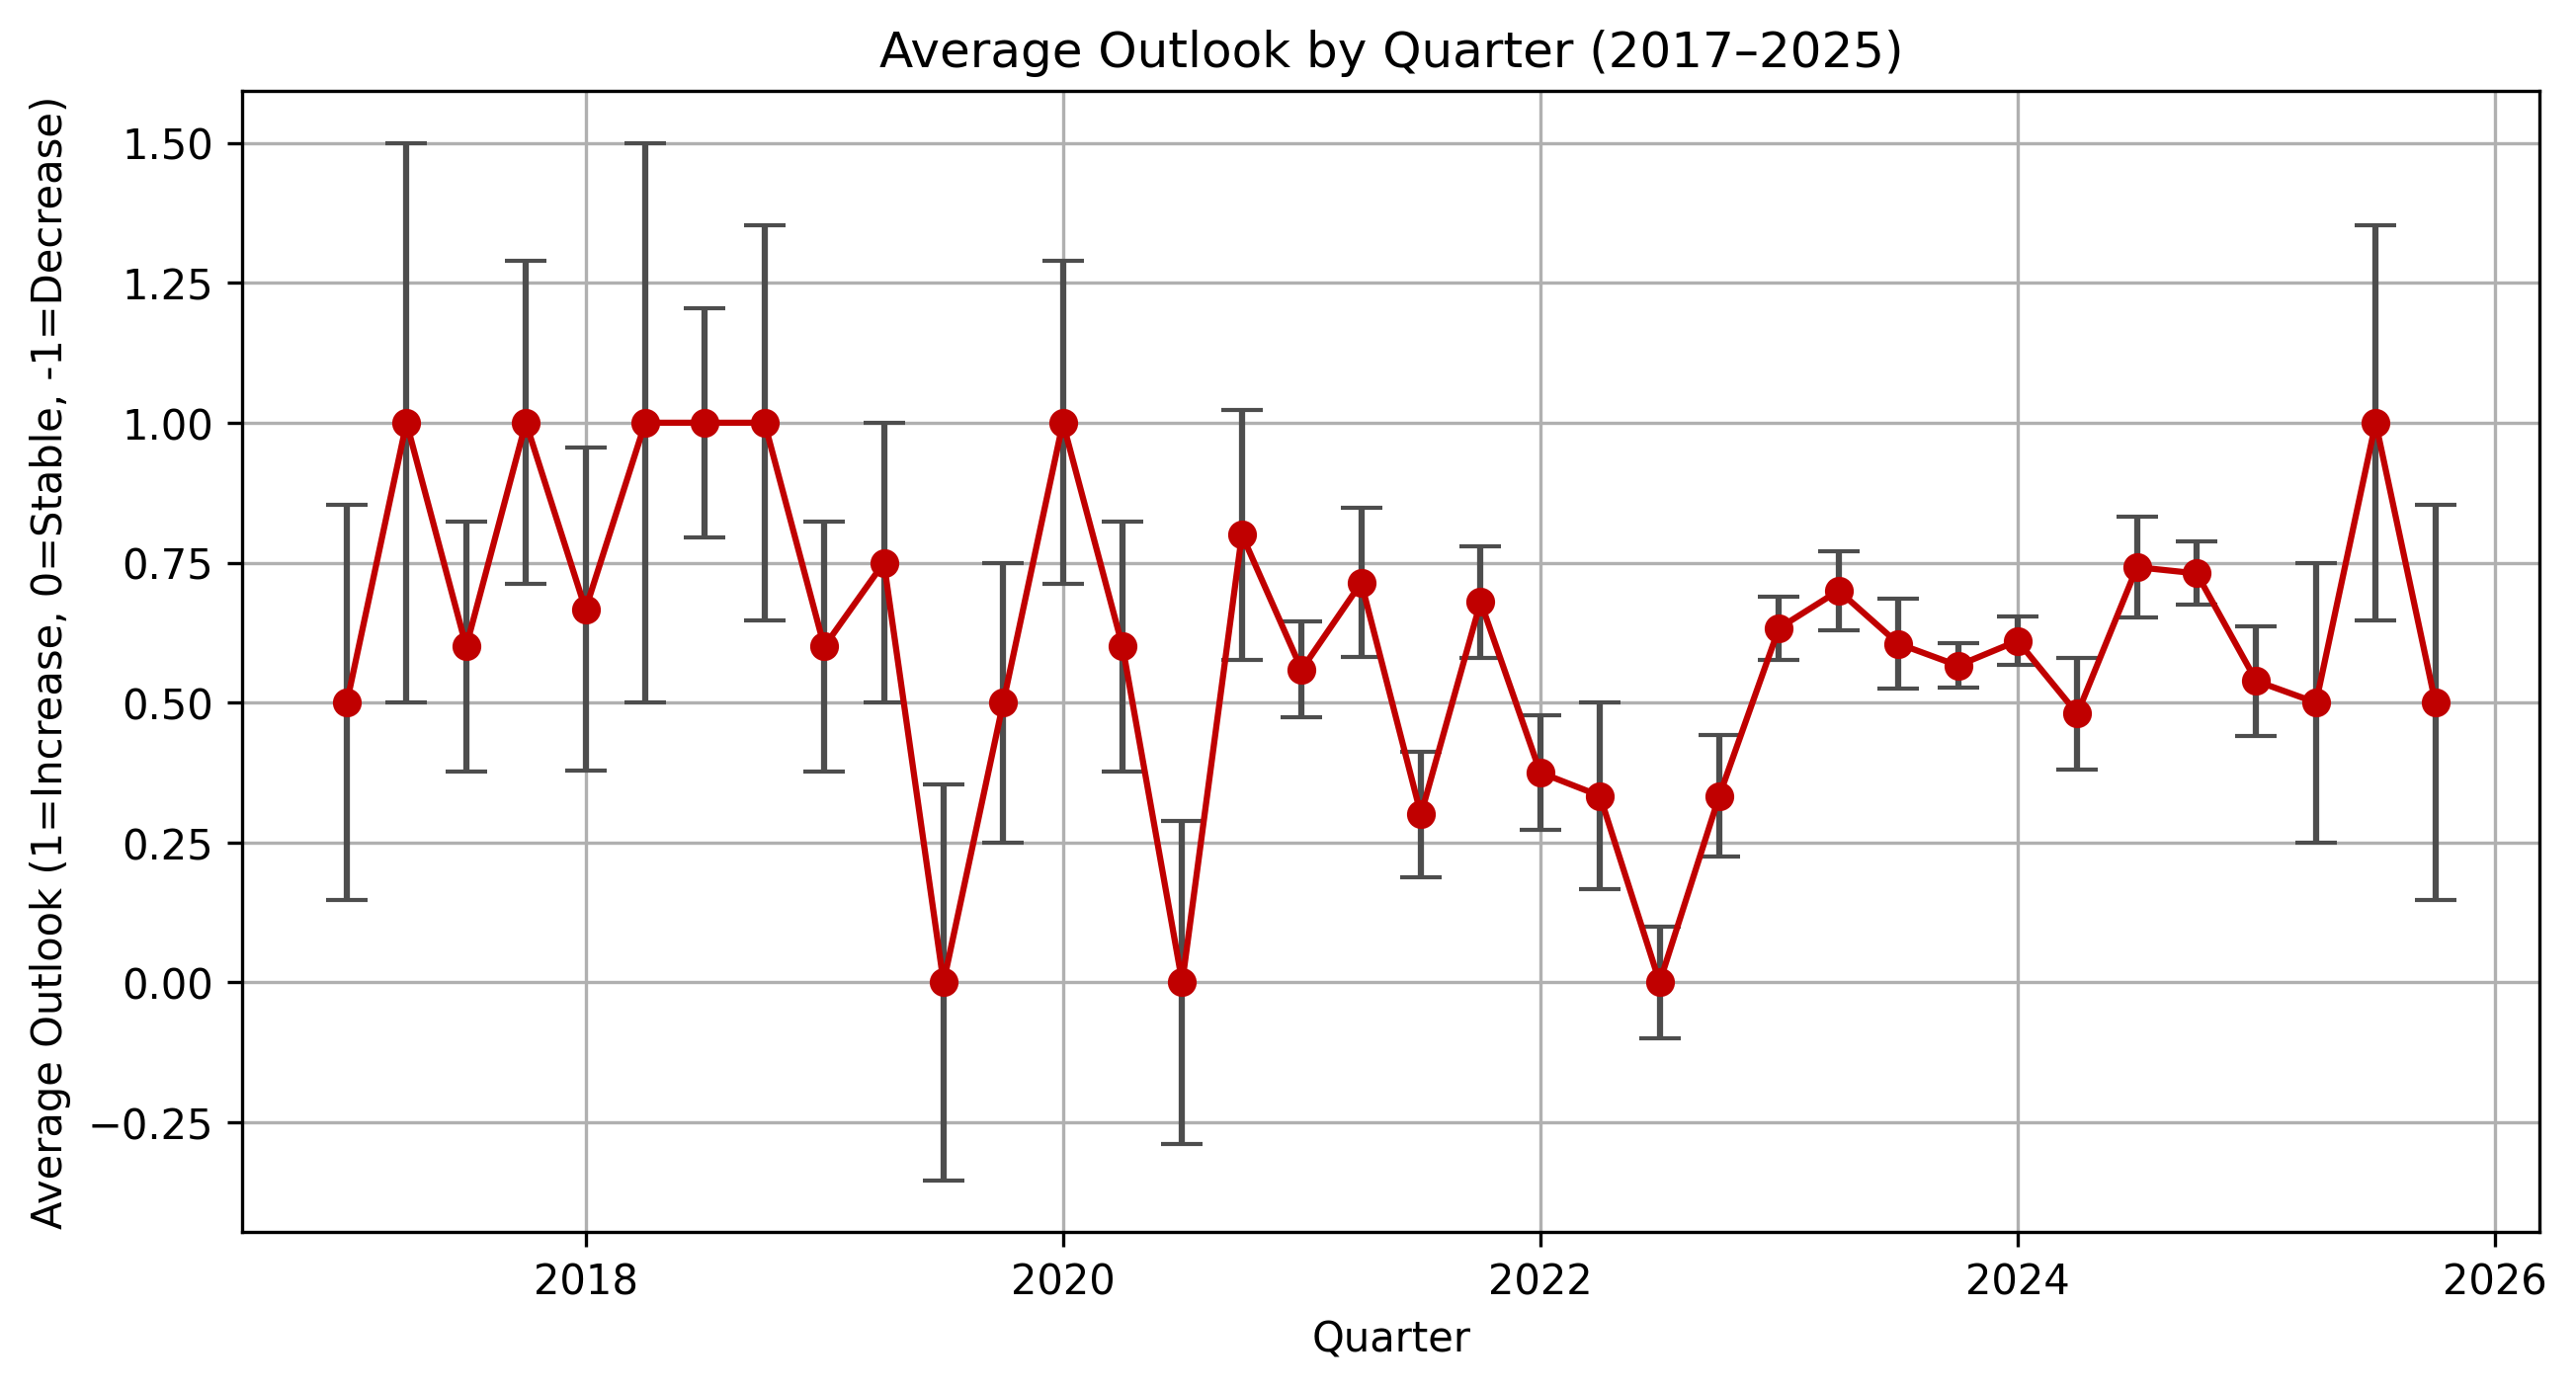
\includegraphics[width=0.7\linewidth]{img/21_TPG}
        \caption{Quarterly aggregation for the sentiment index for the \textit{TPG} GP. Error bar sizes are inversely proportional to the number of available data entries for each quarterly point.}
        \label{fig:21_TPG}
    \end{figure}

    Finally, after filtering points with too few observations, an OLS regression is run on the actual data that the index is meant to represent.
    The results of the regression using yearly aggregation, reported in Table~\ref{tab:ols_sentiment}, show a considerable and significant collinearity between the index and the actual data.

    \begin{table}[h!]
        \centering
        \begin{tabular}{lcccc}
        \toprule
         & Coef.
         & Std.
         Err.
         & t & P$>|t|$ \\
        \midrule
        \textbf{const} & 0.6471 & 0.037 & 17.614 & 0.000 \\
        \textbf{rel\_change\_net\_cf} & 0.5885 & 0.117 & 5.038 & 0.015 \\
        \midrule
        \multicolumn{5}{l}{\textit{Observations}: 5, \quad \textit{R$^2$}: 0.894, \quad \textit{Adj. R$^2$}: 0.859} \\
        \multicolumn{5}{l}{\textit{F-statistic}: 25.38 (p = 0.015), \quad \textit{DW}: 1.873} \\
        \bottomrule
        \end{tabular}
        \caption{OLS Regression of Sentiment on Net Cashflow Changes}
        \label{tab:ols_sentiment}
    \end{table}

    \begin{figure}
        \centering
        \includegraphics[width = 0.7\linewidth]{img/21_TPG_Lagged Sentiment vs Relative Change in Net Cashflow (TPG)}\\
        \caption{Comparison between the sentiment index and the data from Preqin}
        \label{fig:sentiment_TPG}
    \end{figure}

\section{Panel Regression}

\section{Confidence of Results}
    \begin{figure}
        \centering
        \includegraphics[width = 0.4\linewidth]{img/21_TPG_outlook_distribution} \quad
        \includegraphics[width = 0.4\linewidth]{img/23_AGM_outlook_distribution}
        \caption{Distribution of outlooks and confidence levels for funds TPG and Apollo Global Management}
        \label{fig:confidence}
    \end{figure}
It can be observed from the distribution of the outlooks and the of the confidence values that, despite majority of the forecasts expect a positive outlook, the confidence of the model in his forecasts remains very low, with the $0-10\%$ confidence bucket taking the majority of observations (ref. Fig. \ref{fig:confidence})


\section{Comparison with Market Baselines}\label{sec:comparison-with-public-market-baselines}

A primary concern is the potential presence of look-ahead bias, meaning the language model may have been trained on the same information later used to construct the sentiment index.
While it is highly unlikely that the model was trained on proprietary Preqin documents, its forecasts could still be influenced by publicly available information covering similar content.
To address this concern, an initial test was conducted by regressing the sentiment index on macroeconomic variables—factors that are almost certainly part of the model's training data.
The results showed no significant correlation (see Table~\ref{tab:ols_market}), suggesting that the index does not simply reflect pre-existing knowledge of macro trends.


\begin{table}[H]
        \centering
        \caption{OLS Regression Results}
        \begin{tabular}{lccc}
        \toprule
        \textbf{Variable} & \textbf{Coefficient} & \textbf{Std. Error} & \textbf{t-Stat (p-value)} \\
        \midrule
        \textbf{const}   & 0.7880 & 0.112  & 7.005 \; (0.000) \\
        \textbf{snp500}  & 0.4859 & 0.495  & 0.981 \; (0.348) \\
        \textbf{irr}     & -1.2399 & 0.820 & -1.513 \; (0.159) \\
        \midrule
        \multicolumn{4}{l}{\textbf{Model Statistics:}} \\
        \multicolumn{4}{l}{R-squared: 0.173 \quad Adj. R-squared: 0.023} \\
        \multicolumn{4}{l}{F-statistic: 1.153 \quad Prob(F-statistic): 0.351} \\
        \multicolumn{4}{l}{Observations: 14 \quad Durbin-Watson: 1.398} \\
        \bottomrule
        \end{tabular}
        \label{tab:ols_market}
    \end{table}



% ===============================

% ===============================

\chapter{Conclusion and Future Work}\label{ch:conclusion-and-future-work}
% ===============================

\section{Key Takeaways}

\begin{figure}
    \centering
    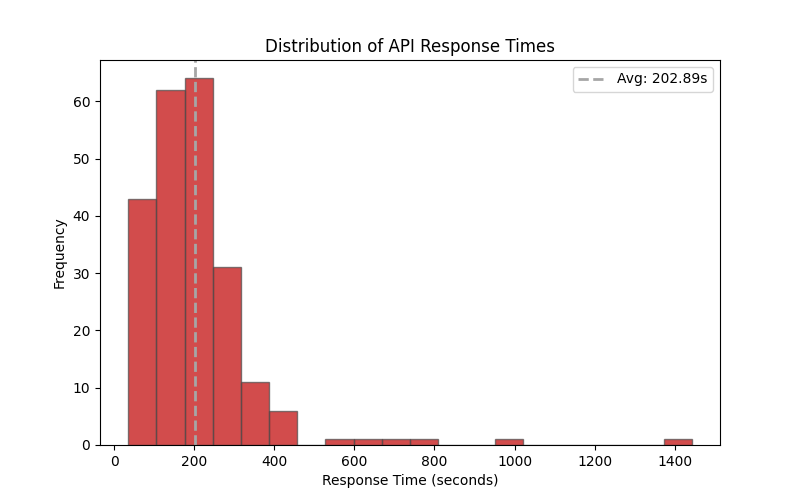
\includegraphics[width=0.8\linewidth]{img/response_time}
    \caption{Average computational time for one query to the LLM. To process 20 thousand documents, 40 thousand queries are required, for a total elaboration time of around 90 days.}
    \label{fig:response_time}
\end{figure}

The proposed methodology demonstrates strong potential when the sentiment index is based on a sufficient number of observations, ensuring that the resulting measure is both stable and representative.
This analysis suggests that in private equity, certain general partners (GPs) appear more consistent in maintaining the expectations they set, while others exhibit greater variability, potentially reflecting differences in communication strategies or internal forecasting accuracy.
However, one critical limitation is computational efficiency: processing large volumes of unstructured text data can become prohibitively time-consuming (see Fig.\ref{fig:response_time} for the average time required to handle just one query) without access to adequate computing resources, especially when applying advanced language models.
Another challenge lies in the heterogeneity of the dataset.
Mixing funds across asset classes and incorporating statements from both GPs and limited partners (LPs) can introduce noise, making it harder to draw clear causal inferences. 
This highlights the importance of segmenting the analysis by fund type, region, or strategy to improve robustness and interpretability.
Despite these limitations, the methodology is highly promising.
It is inherently scalable and can be adapted to a wide range of applications, from monitoring market sentiment in real time to enhancing risk models for capital allocation.
As computational infrastructure improves and more granular data becomes available, this approach could become a standard tool for analyzing belief formation and expectation management in private markets.

\section{Roadmap for Extension}
    Here I present some extensions to overcome the limitations found in my research.

    \paragraph{Deployment on ULHPC and usage of more advanced models} On the local machine, inference was carried out on an NVIDIA GeForce GTX~1070 GPU with 8\,GB of VRAM (CUDA~12.8), which limited the feasible model size and imposed a maximum context length of 2,048 tokens for Deepseek~8B.
    This required documents to be split into multiple segments for processing.
    In contrast, the ULHPC nodes are equipped with NVIDIA Tesla V100-SXM2 GPUs with 32\,GB of VRAM  (CUDA~12.7), offering four times the memory capacity and significantly greater computational capacity.
    This would enable the use of both Deepseek~8B and larger model such as GPT-OSS~20B with extended context lengths of up to 131,072 tokens, allowing entire documents to be processed in a single pass, thereby reducing preprocessing overhead and improving throughput.
    In particular, it would significantly reduce the computational time needed.

    \begin{lstlisting}[style=cmd,label={lst:gptoss}]
        Model
            architecture        gptoss
            parameters          20.9B
            context length      131072
            embedding length    2880
            quantization        MXFP4

        Capabilities
            completion
            tools
            thinking

        Parameters
            temperature    1

        License
            Apache License
            Version 2.0, January 2004
    \end{lstlisting}

    \paragraph{Investigate other quantities and other forecasting horizons} This research was limited to forecasting changes in distribution cashflows in the next year.
    With better hardware and more time to experiment, it will be possible to ask about other quantities, such as returns and fundraising, and different time horizons, such as the next quarter, or the next 2 years.

    \paragraph{Improve Granularity} While the aggregation per GP provides an immediate overview of the performance of its funds, in reality it often aggregates funds from different asset classes (such as Buyout, Venture Capital, Real Estate and Fund of Funds) which often perform in very different ways.
    Moreover, there are other important factors that influence the performances of a fund, for instance the Vintage effect, i.e. the years since its inception which determine at which stage of its life the fund is.
    Therefore, it would be more appropriate to create indices for each fund and then aggregate appropriately per GP or Asset Class.

% ===============================
\appendix

% ===============================
\appendix
\chapter{Appendices}
% ===============================

\section{Additional Tables and Figures}
    In this section I include additional figures.
    \begin{figure}
        \centering
        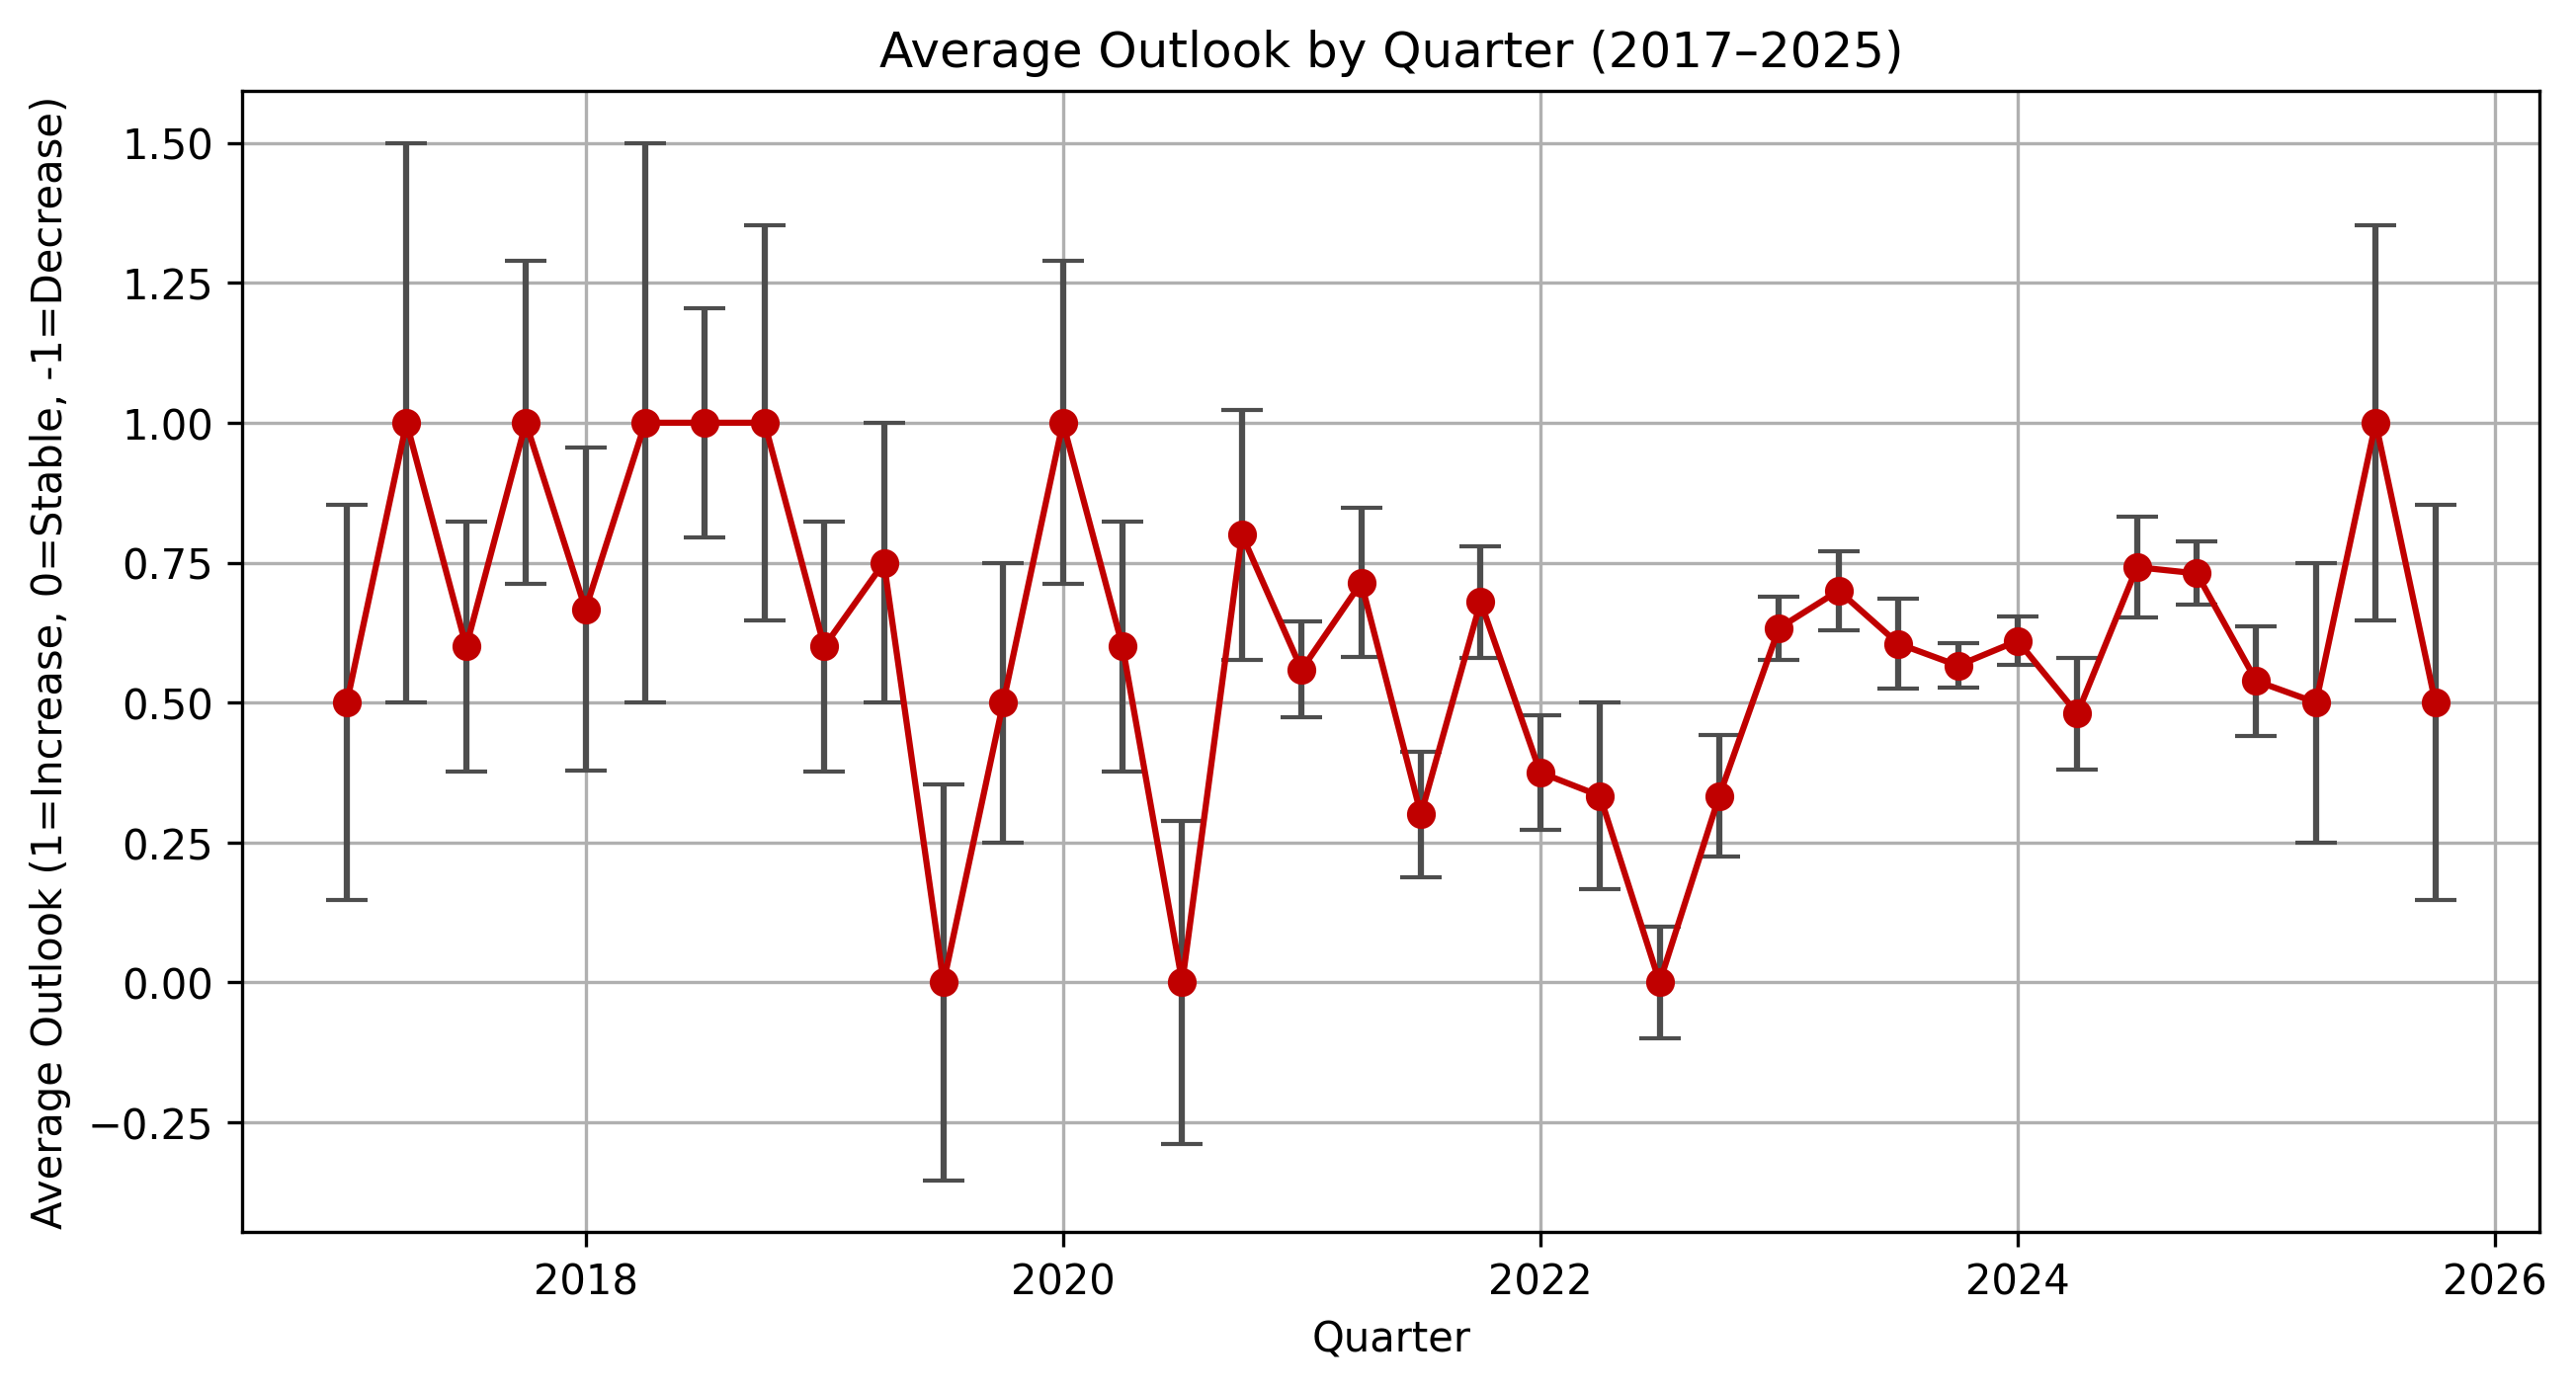
\includegraphics[width = 0.85 \linewidth]{img/21_TPG}
        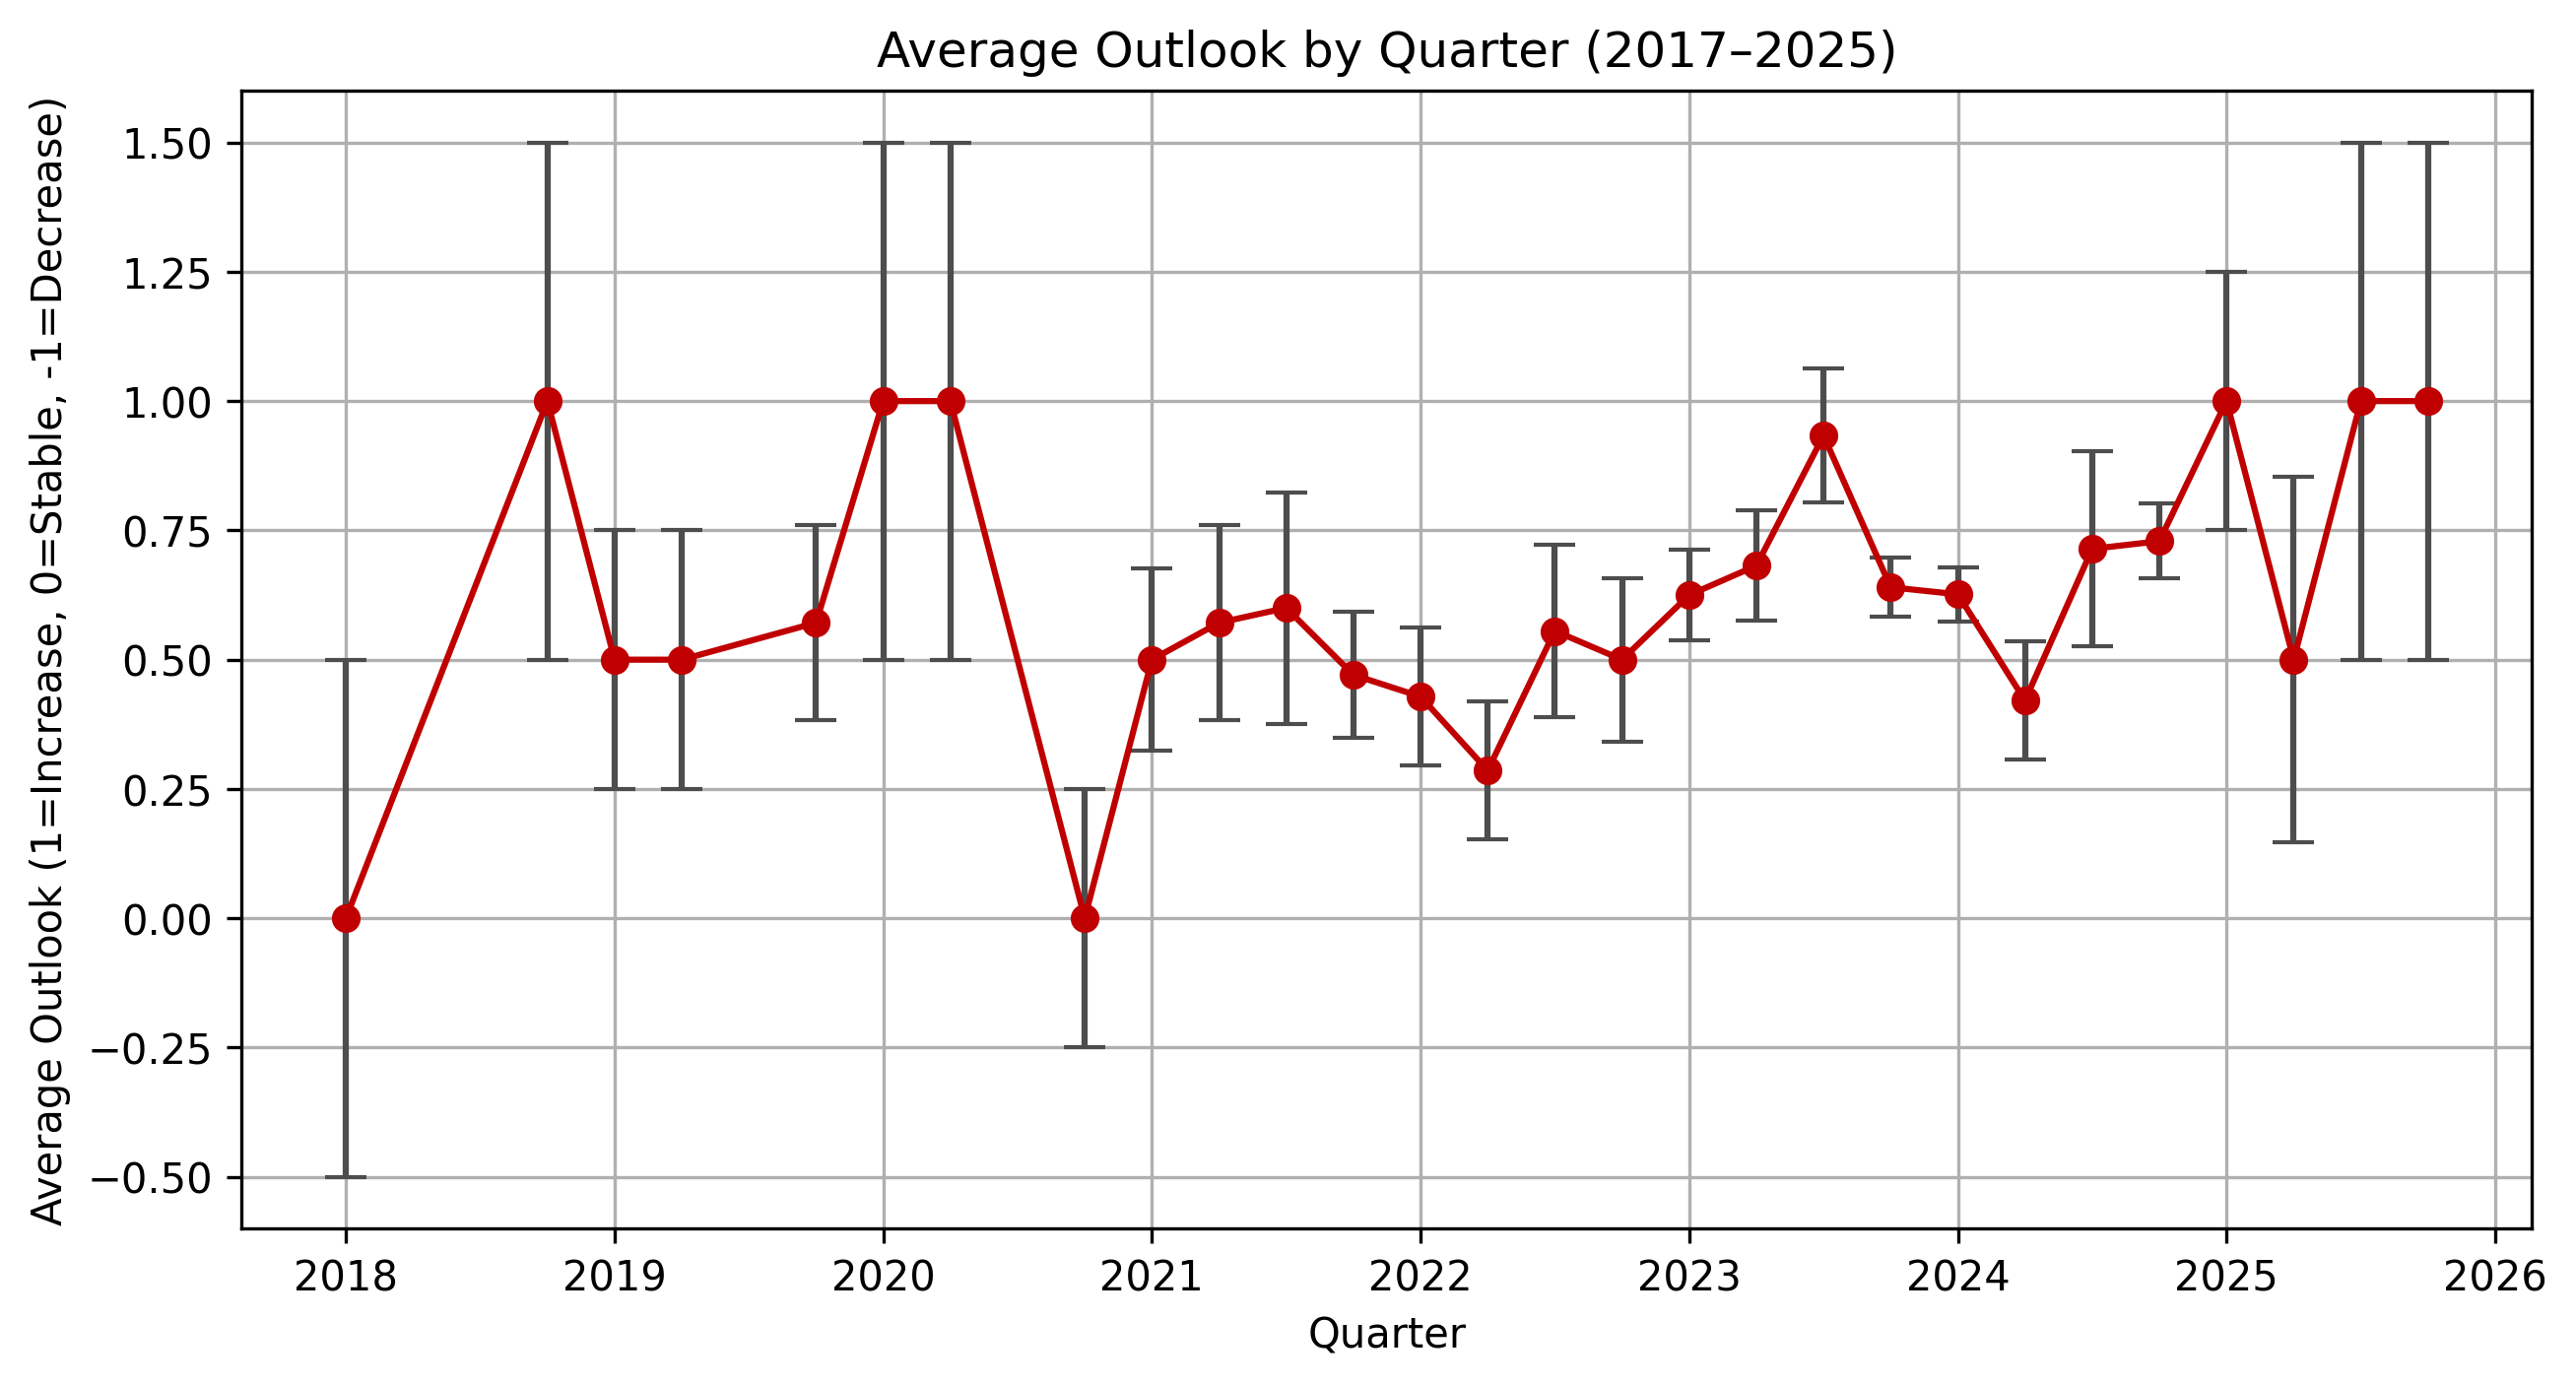
\includegraphics[width = 0.85 \linewidth]{img/22_TCG}
        \includegraphics[width = 0.85 \linewidth]{img/23_AGM}
        \label{fig:figure}
        \caption{The sentiment indices for TPG, Carlyle Group and Apollo Global Management. Quarterly aggregation.}
    \end{figure}

\bibliographystyle{apalike}
\bibliography{references}  % Create references.bib file

\end{document}
